\documentclass{article}
\usepackage{graphicx} % Required for inserting images
\usepackage[utf8]{inputenc}
\usepackage{hyperref}
\usepackage{geometry}
\usepackage{setspace}
\usepackage{listings}
\usepackage{titlesec}
\setlength\parskip{1.5ex}
\usepackage{float}
\usepackage{lipsum}
\usepackage{amsmath}
\usepackage{matlab-prettifier}
\usepackage{amsmath}
\usepackage{bm}

% Set margins and paper size
\geometry{
  top=1.7cm,   
  bottom=1.7cm,
  left=4cm,
  right=4cm,
}
% Set line spacing
\onehalfspacing





%% Operatorer
\newcommand{\diff}{\mathop{}\!\mathrm{d}}
\DeclareMathOperator{\im}{im}
\DeclareMathOperator{\rank}{rank}
\DeclareMathOperator{\E}{E}
\DeclareMathOperator{\Var}{Var}
\DeclareMathOperator{\Cov}{Cov}


%% Nye kommandoer for mengder
\newcommand{\N}{\mathbb{N}}   % Naturlige tall
\newcommand{\Z}{\mathbb{Z}}   % Heltall
\newcommand{\Q}{\mathbb{Q}}   % Rasjonale tall
\newcommand{\R}{\mathbb{R}}   % Reelle tall
\newcommand{\C}{\mathbb{C}}   % Komplekse tall
\newcommand{\A}{\mathbb{A}}   % Affint rom
\renewcommand{\P}{\mathbb{P}} % Projektivt rom


%% Nye kommandoer for vektorer
\renewcommand{\a}{\mathbf{a}}
\renewcommand{\b}{\mathbf{b}}
\renewcommand{\c}{\mathbf{c}}
\renewcommand{\v}{\mathbf{v}}
\newcommand{\w}{\mathbf{w}}
\newcommand{\x}{\mathbf{x}}
\newcommand{\y}{\mathbf{y}}
\newcommand{\z}{\mathbf{z}}
\newcommand{\0}{\mathbf{0}}
\newcommand{\1}{\mathbf{1}}



%% Matematikk
\usepackage{amssymb}   % Ekstra symboler
\usepackage{amsthm}    % Teoremaktige omgivelser
\usepackage{thmtools}  % Teoremaktige omgivelser
\usepackage{mathtools} % Fonter og omgivelser for matematikk
\usepackage{mathrsfs}  % Scriptfont med \mathscr{}
\usepackage{amsmath}

%\usepackage[round]{natbib}
%% Bibliografi
%\usepackage{biblatex} 
%\addbibresource{Source.bib}
\usepackage[backend=biber]{biblatex}
\addbibresource{Source.bib}

\begin{document}

\title{Project 2 - Classification and Regression, from linear and logistic regression to neural networks}
\author{Arangan Subramaniam \& Krithika Gunesegaran}
\date{\today}
\maketitle




\begin{figure}[h]
    \centering
    
\includegraphics[width=7cm]{UiO-kopi.png}
    \label{fig:uio}
\end{figure}


\clearpage

\tableofcontents
\clearpage


\begin{abstract}


This study investigates the effectiveness of various machine learning algorithms in regression and classification tasks, focusing on optimization methods and neural networks. Building on previous regression analysis work with Ordinary Least Squares (OLS) and Ridge Regression, we incorporate Gradient Descent (GD), Stochastic Gradient Descent (SGD), and adaptive optimization techniques to improve model training efficiency. Additionally, we develop a Feed-Forward Neural Network (FFNN) for comparative analysis, exploring the impact of different activation functions on performance. For regression tasks, Ridge Regression performed best, with the lowest prediction error and the highest \( R^2 \) scores, due to its regularization feature that helps prevent overfitting. For classification, Scikit-Learn’s Logistic Regression model was the most accurate and reliable, doing better than both the custom Logistic Regression and the FFNN. This study underscores the importance of tuning hyperparameters like learning rate and regularization strength for model stability and generalization, and offers insights into the practical advantages and limitations of each method. 
\end{abstract}


\section{Introduction}


Machine learning has become a powerful tool for solving diverse real-world problems, ranging from predicting housing prices to diagnosing diseases \cite{charotamine2024}. Understanding how different models behave, how to effectively train them, and how to select the best approach for a given problem is crucial for leveraging the full potential of machine learning. This study focuses on these core aspects by exploring both regression and classification methods, using traditional models as well as neural networks. 


In this study, we build upon our previous study in regression analysis, where we implemented methods like Ordinary Least Squares (OLS) and Ridge Regression to model relationships in data. This time, we extend our focus to include optimization methods, such as Gradient Descent (GD) and Stochastic Gradient Descent (SGD), and evaluate their effectiveness in training models. %The first part of the project focuses on regression, comparing the predictive performance of neural networks to the linear models we previously studied. In the second part, we tackle classification tasks, using logistic regression and our FFNN to classify the Wisconsin Breast Cancer dataset, aiming to distinguish between malignant and benign tumors.

The report is organized as follows: First, we cover the theoretical background, including linear models, optimization techniques, and the basics of neural networks. Then, we describe how we developed and implemented these methods, focusing on building the Feed-Forward Neural Network and setting up key training parameters like learning rates, batch sizes, and epochs. After that, we present the results for both regression and classification tasks, comparing the different approaches. Finally, we summarize our findings, discussing the strengths and weaknesses of each model and point out which methods are best suited for handling complex data.

This study builds on our previous work while providing a practical approach to understanding the complexities of machine learning model development. It allows us to explore the effects of optimization strategies and activation functions. This gives us practical insights crucial for tackling both regression and classification challenges.



\section{Theory}

In this section, we provide an overview of the theoretical concepts applied throughout this study.

\subsection{Linear Regression}

Linear Regression is a statistical model used to predict the value of a dependent variable based on the values of one or more independent variables \cite{ibm_linear_regression}. It is one of the simplest and most widely used methods for fitting continuous functions to data. The linear regression model can be expressed as:
\begin{equation}
    \bm{y} = \bm{X} \beta,
\end{equation}
where \(\bm{y}\) is the vector of observed values, \(\bm{X}\) is the design matrix containing the input data, and \(\beta\) represents the parameters to be estimated. 

To find the best fitting parameters \(\beta\), we minimize a cost function \(C(\beta)\) that measures the differences between the predicted and actual values. In this project, we will focus on two regression methods, Ordinary Least Squares (OLS) and Ridge Regression. The cost function for these regression methods are given in Equation \ref{cost_ols} and \ref{cost_ridge} with their corresponding \(\beta\) when we minimize the cost function in Equation \ref{beta_ols} and \ref{beta_ridge}. 

   \begin{equation}
       C_{\text{OLS}}(\beta) = \frac{2}{n} \| y - X\beta \|_2^2,
       \label{cost_ols}
   \end{equation}
where \(\beta\) is given as, 
   \begin{equation}
       \beta_{\text{OLS}} = (\bm{X}^T \bm{X})^{-1} \bm{X}^T \bm{y}.
       \label{beta_ols}
   \end{equation}

Ridge Regression is like OLS but adds a regularization term to penalize large coefficients to improve the stability of the data. 

\begin{equation}
       C_{\text{Ridge}}(\beta) = \frac{1}{n} \| y - X\beta \|_2^2 + \lambda \| \beta \|_2^2,
       \label{cost_ridge}
\end{equation}
where \(\beta\) is 
\begin{equation}
       \beta_{\text{Ridge}} = (\bm{X}^T \bm{X} + \lambda \bm{I})^{-1} \bm{X}^T \bm{y}.
       \label{beta_ridge}
\end{equation}

\(\lambda\) is the regularization parameter in Ridge Regression that controls the strength of the penalty on \(\beta\). 








\subsection{Logistic Regression}


Logistic Regression is a statistical method primarily used for binary classification, where it predicts the probability that an input belongs to one of two classes, like 0 or 1 \cite{wikipedia_logistic_regression}. Unlike linear regression which predicts continuous outcomes, logistic regression predicts a probability between 0 and 1, showing how likely it is that the given data point falls into a particular class.

The logistic function, also called as sigmoid function, is central to logistic regression. This function is defined as: 

\begin{equation}
    p(t) = \frac{1}{1 + e^{-t}}
    \label{logistic_function}
\end{equation}
where \(t\) is a linear combination of the input features. 
\begin{equation}
t = \beta_0 + \beta_1 x_1 + \beta_2 x_2 + \dots + \beta_n x_n
\end{equation}

Here, \( \beta_0 \) is the intercept, and \( \beta_i \) are the weights for each feature \( x_i \). This transformation guarantees that the output is always between 0 and 1, making it useful for predicting probabilities. 




In binary classification, the probability that a data point \( x_i \) belongs to class 1 can be modeled by using Equation \ref{log_binary}.
\begin{equation}
p(y_i = 1 | x_i, \beta) = \frac{e^{\beta_0 + \beta_1 x_i}}{1 + e^{\beta_0 + \beta_1 x_i}}
\label{log_binary}
\end{equation}

Where \( \beta_0 \) is the intercept, and \( \beta_1 \) is the feature weigths. The (\( \beta \)) parameters helps us determine the  best fit data, by using methods like Gradient Descent (which will be explained further in this report) or other optimization techniques that minimizes the cost function.



The cost function used in logistic regression, given in Equation \ref{cost_log}, measures the error between the predicted probability and the actual class label for each data point. Typically, logistic regression uses the cross-entropy loss, which is minimized to achieve the best model fit.

\begin{equation}
    C(\beta) = -\sum_{i=1}^{n} \left( y_i (\beta_0 + \beta_1 x_i) - \log \left( 1 + \exp (\beta_0 + \beta_1 x_i) \right) \right).
    \label{cost_log}
\end{equation}



Logistic regression serves as an effective soft classifier by outputting a probability for each class, rather than a strict binary output \cite{uke38}. This makes it particularly useful when dealing with data that includes some level of uncertainty. Logistic regression can also be extended to multi-class classification with techniques like "one-vs-all", making it a good choice for many classification tasks because it is easy to use and understand. During this project, we will only be focusing on single-layer classification. 


 


\subsection{Gradient Descent}

Gradient descent (GD) is a widely used optimization algorithm for training machine learning models and neural networks. It works by minimizing the errors between the models predictions and the actual outcomes \cite{ibm_gradient_descent}.


The idea behind Gradient Descent is to minimize a function \(F(x)\), \(x\) = \((x_1, \dots, x_n)\) by iterating the parameters in the direction that decreases the functions value the fastest, which is the negative gradient \(-\nabla F(\mathbf{x})\). This way, the algorithm moves step-by-step towards the lowest point, of the function. This is mathematically expressed in Equation \ref{gradient_descent}. 

\begin{equation}
    \mathbf{x}_{k+1} = \mathbf{x}_k - \eta_k \nabla F(\mathbf{x}_k)
    \label{gradient_descent}
\end{equation}


where \( x_k \) is the current parameter value, \( \eta_k \) is the learning rate, also called as step size and \( \nabla F(x_k) \) is the gradient of the function at point \( x_k \). For every iteration the algorithm moves towards the minimum of the function, reducing the functions value at each step. 

The learning rate \( \eta_k \) is crucial in the gradient descent process. \( \eta_k \) controls how big step you take in the direction of the negative gradient. If the learning rate \( \eta_k \) is too small, the algorithm converges  very slowly while if it is too large, the method may fail to converge or behave erratically. 

For each iteration, the algorithm updates the parameters to move closer to a minimum, effectively decreasing the functions value at each step.




While Gradient Descent (GD) is powerful, it has several limitations. Ideally, GD aims to reach the global minimum, but in non-convex functions, it can get stuck in local minima. Its performance is also highly sensitive to the initial starting point and learning rate. If \(\eta\) is too small, it leads to slow convergence, while a large one may cause divergence. Additionally, computing gradients for large datasets is costly, and the method struggles with saddle points, slowing down the optimization process. 




\subsubsection{Stochastic Gradient Descent}


Stochastic Gradient Descent (SGD) is a variant of Gradient Descent that updates the models parameters more frequently by using just one data point, or a small batch at a time, instead of the entire dataset \cite{uke39}.
In SGD, the models parameters are updated after calculating the gradient for each individual point, rather than waiting for the entire dataset. This means the parameters are updated right away after each training example, instead of waiting until the entire dataset has been processed.
The main idea of SGD is that the cost function we want to minimize can be expressed as the sum of smaller parts, each part corresponding to a data point as in Equation \ref{cost_sgd}.
\begin{equation}
  C(\beta) = \sum_{i=1}^{n} c_i(\bm{x}_i, \beta)
\label{cost_sgd}  
\end{equation}
This also means the gradient can be computed as a sum of the gradients for each data point as in Equation \ref{cost_sgd_gradient}.
\begin{equation}
   \nabla_{\beta} C(\beta) = \sum_{i=1}^{n} \nabla_{\beta} c_i(\bm{x}_i, \beta)
   \label{cost_sgd_gradient}
\end{equation}
This lets SGD calculate and update the gradient more often by using each data point individually, rather than waiting for the whole dataset.

Since SGD updates the model parameters frequently, it allows for quicker and more refined adjustments. However, this frequent updating also have noise, which can cause the parameter updates to fluctuate. While these fluctuations might slow down the convergence, they are also beneficial by adding randomness that prevents the model from getting stuck in local minima, and can increase the chances of finding a global minimum.










\subsubsection{Batches and mini-batches}

Batches computes the total error across the entire training set before updating the model's parameters \cite{ibm_gradient_descent}. While this approach is stable and efficient for smaller datasets, it becomes slow and memory-intensive for large datasets since all data must be processed and stored at once. It produces smooth convergence but can sometimes get stuck in local minima.


Mini-Batches offers a middle ground between batch and SGD by splitting the dataset into smaller batches \cite{ibm_gradient_descent}. After each mini-batch is processed, the model updates its parameters. This approach combines the stability of batches with the frequent updates of SGD. This approach is more efficient and makes it well suited for large datasets. Typically, each batch contains a few hundred to a few thousand data points, allowing the model to learn efficiently without processing the entire dataset at once.


\subsubsection{Momentum parameter}

Momentum is a technique used in Gradient Descent to speed up convergence by using the information from previous iterations. Instead of just using the current gradient, momentum also uses parts of the previous update to smooth out changes and help the optimization move faster in steady directions. This speed, the momentum update, can be describes as:

\begin{equation}
    v_t = \rho v_{t-1} + \eta \nabla_\theta E(\theta_t),
\end{equation}
where \( v_t \) is the momentum term, \( \rho \) is the momentum parameter, ranging between 0 and 1. The momentum term controls how much of the past velocity is kept. \( \eta \) is the learning rate and \( \nabla_\theta E(\theta_t) \) is the gradient of the error function with respect to the current parameters.



Once the velocity \( v_t \) is calculated, the parameter update is done as follows:

\begin{equation}
    \theta_{t+1} = \theta_t - v_t
\end{equation}

Momentum helps the algorithm continue moving in the same direction, making it more efficient and faster in finding the minimum, especially in places where the cost function is relatively flat. The momentum parameter \(\rho\) and learning rate \(\eta\) can be defined as: 

\begin{equation}
    \rho = \frac{m}{m + \mu \Delta t},
\end{equation}
and
\begin{equation}
    \eta = \frac{(\Delta t)^2}{m + \mu \Delta t},
\end{equation}

where \( m \) is the mass, \( \mu \) is the viscous drag and \( \Delta t \) is the time step.

Here, the parameter \(m\) works like the mass of a particle, giving it inertia. This means it helps the optimization process keep moving in the same direction, even when conditions change, resulting in smoother and more efficient movement through flat regions of the cost function. Similarly, the viscous drag \(\mu\) works like a resistance and slows down the movement. 

Overall, adding momentum makes the optimization process smoother and more efficient, even in areas that are noisy or have steep gradients, leading to faster convergence and better results.





\subsubsection{AdaGrad}

Adaptive Gradient Algorithm (AdaGrad) is an optimization technique used in machine learning to adjust the learning rate for each parameter during training, making it particularly effective \cite{soni_adagrad_2023}. AdaGrad automatically adapts the learning rate for each parameter based on past updates, leading to more efficient convergence \cite{soni_adagrad_2023}. AdaGrad works by scaling the learning rate for each parameter based on the sum of its past squared gradients. 




\subsection{Adam Optimizer \& RMSprop}

Second-order moment methods like Adam and RMSprop adaptively adjust the learning rate based on both the gradient and the curvature of the error surface. This allows them to better navigate complex error landscapes.
Adam combines the running averages of both gradients and their squares to adapt the learning rate dynamically. This makes it particularly effective for handling noisy data and sparse gradients.

RMSprop focuses on adjusting the learning rate by keeping a moving average of the squared gradients \cite{uke39}. This helps stabilize and speed up convergence, especially in scenarios with uneven error landscapes. 

These adaptive techniques make both optimizers well-suited for efficiently training deep learning models.



\subsection{Neural networks}

Neural Networks are computational models inspired by biological neural networks in the human brain. They learn from examples without being explicitly programmed with task-specific rules. This is usually done by using training and test data.  Neural networks are built from layers of connected neurons. The concept is that each neuron takes in multiple inputs, combines them using weights, applies a function to decide its output, and then sends this output to the next layer. The strength of the connections between neurons is represented by weights. By adjusting these weights, the network learns to recognize patterns and improve its performance on a specific task. This can be mathematically expressed as: 


\begin{equation}
     y = f\left(\sum_{i=1}^{n} w_i x_i\right) = f(z), 
     \label{neural1}
\end{equation}
Where \( y \) is the output, \( w_i \) are the weights, \( x_i \) are the input signals, and \( f(z) \) is the activation function.





\subsubsection{Feed-Forward Neural Network (FFNN)}

This is the simplest type of Neural Network, where the input only flows in one direction from input to output, without looping back \cite{neuralnetworks_MH}. Each layers nodes are connected to all nodes in the next layer, which makes the network fully connected. 

The model have three types of layers: the input layer, hidden layers and output layer. Each neuron takes its inputs, calculates a weighted sum, applies an activation function, and then sends the result to the next layer, just like in a neural network. This can be mathematically expressed as: 
\begin{equation}
    z = \sum_{i=1}^{n} w_i x_i, 
\end{equation}
Where \( z \) is the weighted sum, \( w_i \) are the weights, \( a_i \) are the inputs to this neuron.
The neurons output \( y \) is calculated by applying an activation function \( f\) to the input \( z \). 
\begin{equation}
    y = f(z)
\end{equation}

In a FFNN, using this function creates a perceptron. It is when it takes in one or more inputs, applies weights to them, and then gives a result of either 1 or 0. It works well for binary classification tasks, where it can be used in the output layer to separate two classes.

In a neural network, each layer receives input signals either from the original input data or from the outputs of neurons in the previous layer. To make the model more flexible, a bias term is added to each neurons weighted sum. This allows the network to have a threshold that can shift, making the model more capable of fitting a wider range of functions.

The input to the activation function for neuron \( j \) in a layer can therefore be expressed as in Equation \ref{ffnn_bias}.

\begin{equation}
    z_j = \sum_{i=1}^{n} w_{ij} a_i + b_j,
    \label{ffnn_bias}
\end{equation}
where \( z_j \) is the pre-activation output of neuron \( j \), \( w_{ij} \) is the weight associated with the connection between input \( i \) and neuron \( j \).\( a_i \) is the input to the neuron, coming from the previous layer or the input layer and \( b_j \) is the bias term for neuron \( j \).

The bias \( b_j \) allows the neuron to produce an output even if the sum of weighted inputs is zero. This flexibility is crucial as it helps the neuron shift the activation threshold, making it easier for the neuron to activate under different circumstances, depending on the problem being solved.

Thus, the final output of a neuron is calculated by applying an activation function \( f \) to \( z_j \), allowing the network to introduce non-linearity and better capture complex patterns in the data. This is a core mechanism that helps the neural network approximate complex functions and relationships in the data.






\subsubsection{Activation Functions}

Activation functions play a crucial role in enabling neural networks to learn complex patterns by introducing non-linearity \cite{neuralnetworks_MH}. Without non-linear activation functions, neural networks would be limited to performing simple linear transformations, regardless of the number of layers, and unable to model complex data effectively.
We will be focusing on three different activation functions during this project. The sigmoid funtion, Rectified Linear Unit (ReLU) and Leaky ReLU. 

The sigmoid, also called as logistic function is commonly used for binary classification and maps input values to a range between 0 and 1. This is given as Equation \ref{sigmoid}. 
    \begin{equation}
        f(x) = \sigma(x) = \frac{1}{1 + e^{-x}}
        \label{sigmoid}
    \end{equation}

The sigmoid is often used in the output layer of binary classification models to represent probabilities.

The Rectified Linear Unit (ReLU) function is the most widely used activation function in deep learning due to its simplicity and efficiency. It outputs the input directly if it is positive, otherwise it returns zero. This is given as Equation \ref{relu}

\begin{equation}
    R(z) = 
    \begin{cases} 
      0 & \text{if } z \leq 0 \\
      z & \text{if } z > 0 
      \label{relu}
   \end{cases}
\end{equation}


However, ReLU suffers from the dying ReLU problem, where neurons can stop learning entirely by outputting zero for all inputs. This occurs when the weights are adjusted so that the inputs turn negative, effectively "killing" the neuron.

To reduce the this issue, Leaky ReLU allows a small, non-zero output for negative input values, keeping neurons active even when they receive negative inputs. This is given as: 
\begin{equation}
        f(x) = \begin{cases}
            x, & \text{if } x \geq 0 \\
            \alpha x, & \text{if } x < 0
            \label{leakyrelu}
\end{cases}
\end{equation}

Where \( \alpha \) is typically a small value like 0.01.




Choosing the right activation function is crucial for neural network performance. The sigmoid function is effective for binary classification, but it can suffer from vanishing gradients, making it less suitable for deep networks. ReLU, on the other hand, is widely used in hidden layers due to its simplicity and computational efficiency, which generally leads to faster convergence. Leaky ReLU builds on this by addressing the dying ReLU problem, helping to maintain active neurons during training and making it a more robust alternative in some scenarios. 





\section{Implementation}



\subsection{Stochastic Gradient Descent}


We generated sample data using \(n = 100\) observations of \(x\), with \(x\) values randomly sampled from a uniform distribution. To keep the model straightforward, we defined the target variable \(y\) using a simple quadratic function:

\begin{equation}
    y = 1 + 2x + 3x^2 + \epsilon
\end{equation}

where \(\epsilon\) represents noise sampled from a standard normal distribution.                                                      
We then implemented and analyzed gradient descent techniques, each offering different approaches to optimize model convergence. These methods included standard gradient descent, modification with momentum, mini-batch Stochastic Gradient Descent, and adaptive learning rate optimizers. Below is a summary of each technique and its role in enhancing model training efficiency. 



\subsubsection{Plain Gradient Descent}
  %  \item \textbf{Plain Gradient Descent}
The \texttt{PlainGradientDescent} function minimizes Mean Squared Error (MSE) by optimizing model weights (\(\beta\)) through gradient descent, with optional momentum and L2 regularization. In each iteration, it calculates the gradient of the MSE with respect to \(\beta\), adding a ridge penalty term if ridge parameter (\(\lambda\)) is provided. If a nonzero momentum parameter (\(\rho\)) is set, the function applies momentum by incorporating a fraction of the previous update to smooth and speed up convergence, helping the algorithm move past areas where progress is slow. The testing included Ordinary Least Squares (OLS) regression with and without momentum, and Ridge Regression with different values of \(\lambda\) and learning rates (\(\eta\)). Results were visualized with line plots showing MSE of iterations, comparing momentum and non-momentum versions. These results will be presented in the next section. Additional heatmaps displayed MSE in Ridge regression as function of the ridge parameter \(\lambda\) and \(\eta\), highlighting the effects of these parameters on model accuracy and stability. 

\subsubsection{Stochastic Gradient Descent}
  %  \item \textbf{Stochastic Gradient Descent}
The \texttt{StochasticGradient}function performs Stochastic Gradient Descent (SGD) with mini-batches, optional momentum, and L2 regularization for optimizing linear regression models. Each epoch, shuffles the data and divides it into mini-batches of size \(M\), computing the gradient of the Mean Squared Error (MSE) for each batch. With Ridges regularization term  \(\lambda\), a penalty is added, and if momentum \(\rho\) is specified, the function applies a fraction of the previous velocity to smooth and accelerate convergence. This function was tested on Ordinary Least Squares (OLS) and Ridge regression, both with and without momentum, and varying regularization parameters. Results included MSE line plots and heatmaps displaying the effects of batch size, learning rate (\(\eta\)), and ridge penalty (\(\lambda\)) on convergence and model performance. 
    
\subsubsection{Adagrad} 
  %  \item \textbf{Adagrad}
The \texttt{Adagrad\_plain} function applies the Adagrad optimization method, where gradient updates are adjusted based on the squared gradients, making the learning rates apdaptive for each parameter. Optional momentum (\(\eta\)) is included to smooth updated and accelerate convergence, while ridge regularization term (\(\lambda\)) can be added to penalize large weights, helping to control overfitting. At each iteration, MSE is recorded to track model performance over each epoch. MSE was recorded across epochs for each iteration to compare how adaptive learning rates, momentum, and regularization impacted model performance.

The \texttt{Adagrad\_StochasticGradient} function combines Adagrad with mini-batch stochastic gradient descent, shuffling the data at the each epoch and dividing it into mini-batches for efficient processing. The adaptive learning rate scales mini-batch update, and optional momentum and L2 regularization further enhance model stability and generalization. Testing the function for \(\rho\) > 0, \(\rho\) = 0, and regularization demonstrates how these adjustments impact stability, and overall model accuracy, giving insight into which settings best optimize training.  

     \subsubsection{RMSprop and Adam Optimizers}
The \texttt{RMSprop} function implements the RMSprop optimization algorithm, maintaining a running average squared gradients (\texttt{G}) to adaptively adjust the learning rate. A decay factor (\texttt{rho}) helps stabilize convergence, especially in the presence of noisy gradients. The \texttt{Adam} function applies the Adam optimizer, combining momentum (first momentum estimate,\texttt{m}) with adaptive learning rates (second moment estimates, \texttt{v}), and includes bias correction to ensure stable and efficient updates. Both functions have been added to the library for potential future use but have not been tested or applied to any models.
    

\subsection{Neural Network}
The neural network, defined in \texttt{FeedForwardNN.py}, is designed for flexible application in both regression and binary classification tasks. Key parameters include network architecture, learning rate \(\eta\), momentum parameter \(\rho\), and regularization term \(\lambda\), with weights initialized using \(He\) initialization to promote stable gradient flow and biases set to zero for simplicity \cite{HeInitialization}.Even though the He intialization is more favorable for ReLU, we chose sigmoid as the final activation function, affect the outcomes of the results. The reason for He Intialization is to prevent gradient explosion \cite{HeInitialization}. A learning schedule gradually reduce the learning rate, preventing training instability \cite{LearningSchdule}. Forward and backward propagation methods calculate activations and gradients across layers, essential for efficient weight updates and optimization. 
The model is trained via \texttt{fit()} function, which employs Stochastic Gradient Descent algorithms such employing mini-batch with data shuffling to improve convergence and applies momentum to accelerate learning. Cost functions used are Binary Cross-Entropy(BCE)/log loss for classification and Mean Squared Error for regression, with optional regularization \(\lambda\) to control overfitting. Evaluation metrics include accuracy for classification and MSE or \(R^2\) for regression, providing insight into model performance on new data. 

In \texttt{FFNN\_evaluation.ipynb}, we assessed the performance of the model using synthetic polynomial regression data to test accuracy on non-linear pattern. Standardizing the input data to zero mean and unit variance ensures consistent and stable training. The FFNN model is trained and compared with Linear Regression, Ridge Regression, and \texttt{MLPregressor} from Scikit-learn \cite{pedregosa2011scikit}, with MSE calculated for performance comparison. Further analysis on test data uses MSE and \(R^2\) scores to evaluate FFNN performance relative to other models. 


\subsection{Activation Functions}
When testing the Activation Functions, we implemented the custom Feed-Forward Neural Network (FFNN), trained using three activation functions- \texttt{Sigmoid, ReLU, Leaky ReLU}-to analyze their effects on model performance. Each model configuration was trained over 50 epochs with \(\eta\)=0.02, and \(\rho\) = 0.1, using a batch size of 10 for each activation functions. Following training, the code plots the Mean Squared Error (MSE) over epochs for each activation function. This visualization enables comparative analysis of convergence rates and training efficiency across activation functions, providing insights into their distinct impacts on model performance  and error minimization. 

\subsection{Classification}
This implementation trains a Feed-Forward Neural Network (FFNN) for binary classification on \textbf{the breast cancer dataset} from Scikit-learn \cite{pedregosa2011scikit}, using \texttt{.load\_breast\_cancer} method, which includes to differentiate malignant from bening tumors \cite{breast}. Binary Cross-Entropy, also known as Log loss,  is used as the cost function, ideal for classification as it penalizes prediction errors in probability-based outputs \cite{logloss}. The data  is split into 80/20 training and testing sets, then standardized with \texttt{StandardScaler} to achieve zero mean and unit variance \cite{pedregosa2011scikit}, promoting stable and faster convergence. The FFNN model, with a single hidden layer of 10 nodes, is trained using Sigmoid activation, Momentum and Ridge regularization. Training and validation metrics, including accuracy and loss, are recorded across epochs and visualized with smoothed plots for clarity. Accuracy is calculated using the \texttt{accuracy\_score} method from \texttt{sklearn.metrics} \cite{pedregosa2011scikit}. The performance of the model is further analyzed with different \(\lambda\) and \(\eta\) through heatmaps. Finally, the FFNN results are compared with \texttt{MLPClassifier} from Scikit-Learn \cite{pedregosa2011scikit}, to highlight differences in training loss and accuracy under various parameter settings. 

\subsection{Logistic Regression}
The \texttt{LogisticRegression} function uses Stochastic Gradient Descent (SGD) with mini-batches, momentum (\(\rho\)), and L2 regularization (\(\lambda\)) to optimize the weights (\texttt{Beta}). The \texttt{Sigmoid} function transforms continuous values into a range of (0,1), ensuring that input the next layer remains within a fixed range, which stabilizes weight updates and enhances model convergence \cite{AsiRah}. The \texttt{binary\_cross\_entropy\_loss}, using the \texttt{log\_loss} method imported from \texttt{sklearn.metrics}\cite{pedregosa2011scikit}, calculates the difference between predicted probabilities and true labels. This loss function is ideal for logistic regression, as it heavily penalizes misclassifications, encouraging the model to minimize classification errors \cite{Data_science}. Additionally, a learning schedule (\texttt{LearningSchedule}) adjusts the learning rate, improving the stability as the model converges. A grid search is conducted over \(\lambda\) and initial learning rate \(\eta\) values, systematically evaluating their effects on model loss which is visualized in final heatmaps.

\section{Results}

\subsection{Stochastic Gradient Descent}

\begin{figure}[h!]
    \centering
    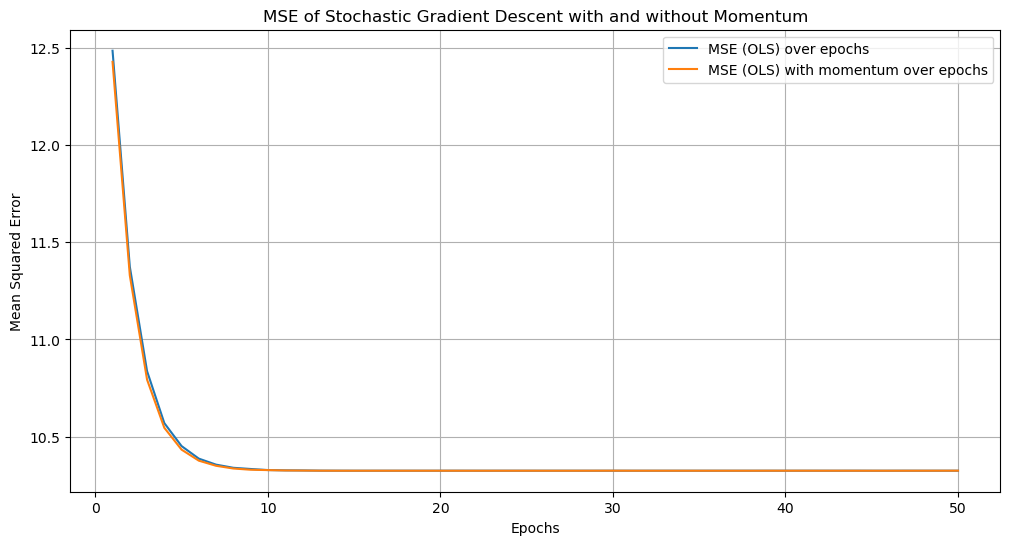
\includegraphics[width=0.9\linewidth]{MSE_OLS_plot_momentum_no_momentum_TaskA.png}
    \caption{MSE of Stochastic Gradient Descent with and without Momentum}
    \label{MSE_OLS_plot_momentum_no_momentum}
\end{figure}


Figure \ref{MSE_OLS_plot_momentum_no_momentum} illustrates the Mean Squared Error (MSE) over epochs for Stochastic Gradient Descent (SGD) with and without momentum, highlighting momentum's impact on optimization. Both methods initially reduce error rapidly, but the model with momentum converges slightly faster and stabilizes at a marginally lower MSE. Momentum smooths out fluctuations caused by noisy updates in SGD by incorporating information from previous updates, allowing the optimization process to progress more stably and efficiently. By the end of 50 epochs, both approaches reach similar MSE levels.
%though the addition of momentum achieves this with improved stability and efficiency, as described in the method section.


\begin{figure}[h!]
    \centering
    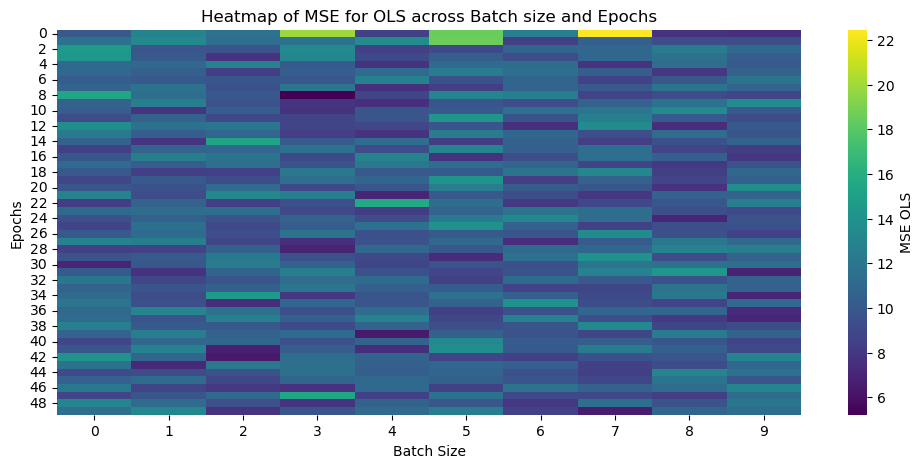
\includegraphics[width=0.9\linewidth]{Epoch_batchsize_TaskA_1.png}
    \caption{Heatmap of MSE for OLS across Batch size and Epochs}
    \label{Epoch_batchsize_1}
\end{figure}


The heatmap, in Figure \ref{Epoch_batchsize_1}, shows the  MSE for Ordinary Least Squares (OLS) across different batch sizes and epochs, illustrating how batch size impacts the training dynamics. Smaller batch sizes introduce more noise, which helps avoid local minima but causes fluctuations in MSE, while larger batches provide smoother, more stable convergence but may get stuck in suboptimal solutions. Mini-batch sizes achieve a balance, combining frequent updates with stability, leading to efficient learning across epochs. Overall, as epochs increase, MSE mostly decreases across batch sizes, reflecting improved model performance.

\begin{figure}[h!]
    \centering
    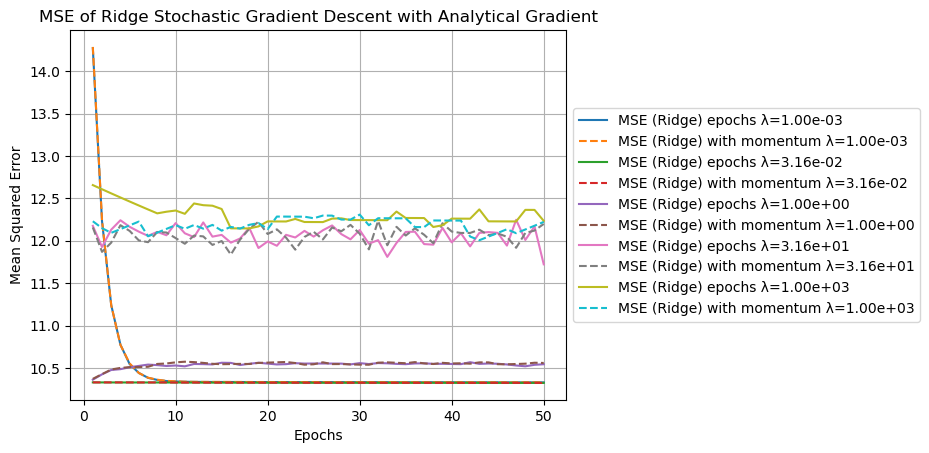
\includegraphics[width=1.2\linewidth]{MSE_Ridge_plot_TaskA_2.1.png}
    \caption{MSE of Ridge Stochastic Gradient Descent with Analytical Gradient}
    \label{MSE_Ridge_plot_TaskA_2}
\end{figure}

Figure \ref{MSE_Ridge_plot_TaskA_2} illustrates MSE over epochs for Ridge Regression with Stochastic Gradient Descent (SGD) using various regularization term (\(\lambda\)) and the option of momentum. Lower \(\lambda\) values like \(1 \times 10^{-3}\) lead to faster convergence and lower MSE, while higher values like \(3.16 \times 10^1\) and \(1 \times 10^3\) cause slower convergence and stabilize at a higher MSE due to stronger regularization. Intermediate values like \(3.16 \times 10^{-2}\) and \(1\times 10^{0}\) balance error reduction with stability. Momentum smooths the convergence path, reducing fluctuations and providing more stability, particularly for higher \(\lambda\) values. Overall, this demonstrates that balancing \(\lambda\) and using momentum can optimize both the stability and speed of the learning process.



\begin{figure}[h!]
    \centering
    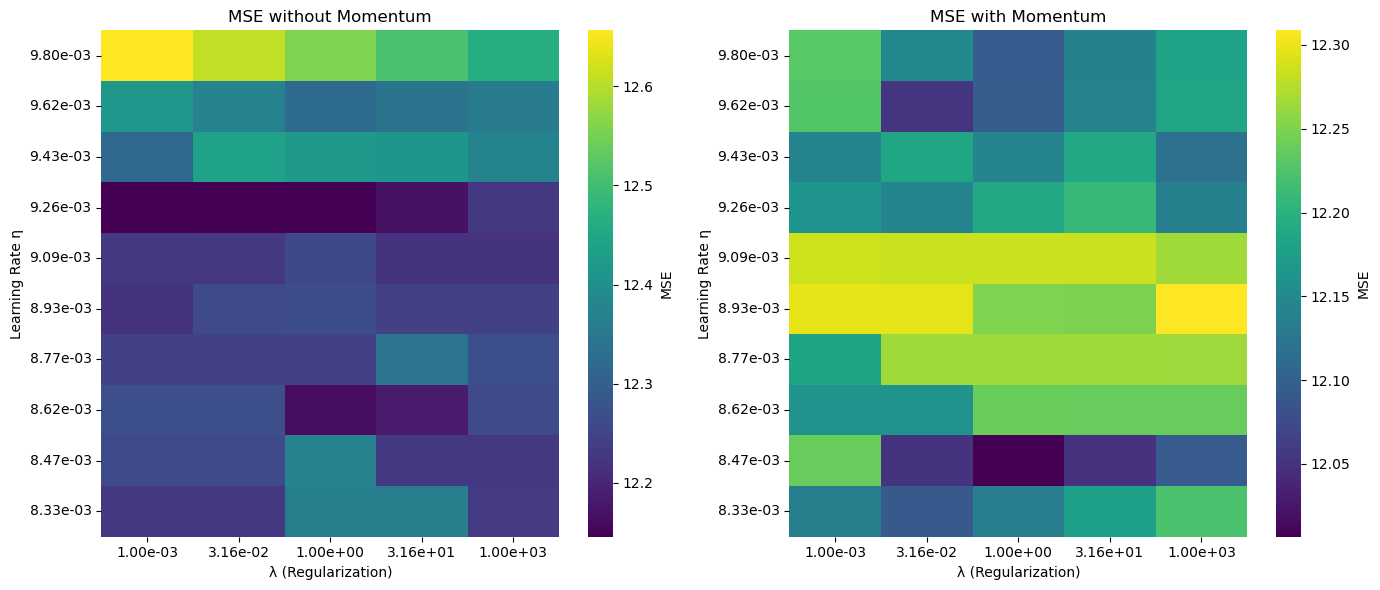
\includegraphics[width=1.2\linewidth]{MSE_Ridge_heatmap_TaskA_2_2.png}
    \caption{Heatmaps of MSE with and without momentum across \(\lambda\) and \(\eta\) }
    \label{MSE_Ridge_heatmap_TaskA_2_2}
\end{figure}



Figure \ref{MSE_Ridge_heatmap_TaskA_2_2} compares the Mean Squared Error (MSE) for Ridge Regression across different combinations of regularization terms (\(\lambda\)) and learning rates (\(\eta\)), both with and without the use of momentum. In the MSE without momentum heatmap, the lowest MSE is achieved with a learning rate of \(9.26 \times 10^{-3}\) and low values of \(\lambda\), which shows that without momentum, a moderate learning rate and low regularization yield the best results. In contrast, the MSE with momentum heatmap reveals that the lowest MSE occurs when the learning rate is \(8.47 \times 10^{-3}\) and \(\lambda\) is between \(3.16 \times 10^{-2}\) and \(3.16 \times 10\). However, overall, the MSE values in the "without momentum" scenario are generally lower, indicating that in this case, the addition of momentum did not improve model performance and led to higher MSE values across most parameter combinations. This suggests that, for this specific task, using Ridge Regression without momentum provided more favorable results in terms of minimizing prediction error.



\subsection{Neural Network}

\begin{figure}[h!]
    \centering
    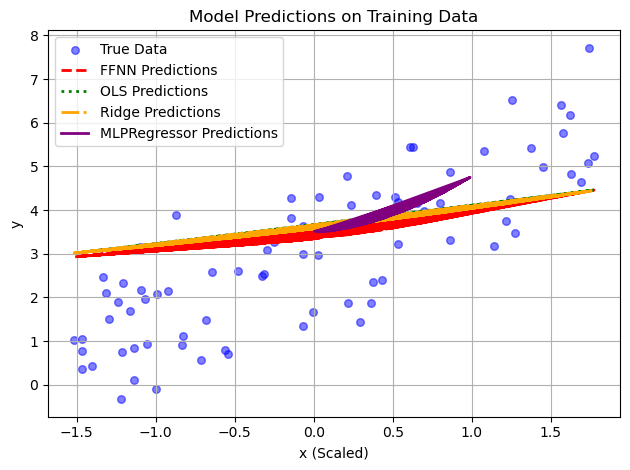
\includegraphics[width=0.9\linewidth]{Results_Obtained_linear_and_NN_code_taskB_1.png}
    \caption{Model Prediction on Training Data}
    \label{Results_Obtained_linear_and_NN_code_taskB_1}
\end{figure}

\begin{figure}[h!]
    \centering
    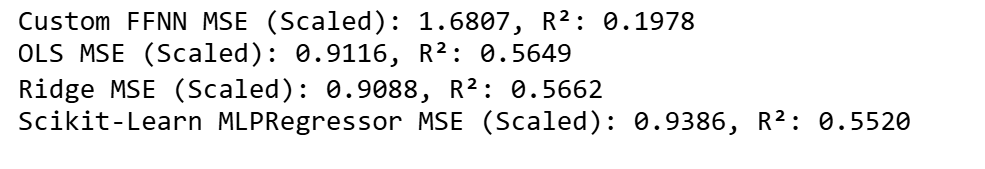
\includegraphics[width=0.7\linewidth]{Values.png}
    \caption{Model Performance Comparison: Mean Squared Error (MSE) and R² Scores for Various Regression Models on Scaled Data}
    \label{values}
\end{figure}




Figure \ref{Results_Obtained_linear_and_NN_code_taskB_1} compares the performance of four models for the MSE and \( R^2 \) score: Ordinary Least Squares (OLS), Ridge Regression, a custom Feed-Forward Neural Network (FFNN), and Scikit-Learn's MLPRegressore. OLS and Ridge Regression both achieve almost identical MSE and \( R^2 \) scores as shown in Figure \ref{values}, showing a stable and solid performance in capturing the data trends. Interestingly, although the MLPRegressor is generally well-suited for capturing non-linear relationships, its MSE is slightly higher than OLS and Ridge, indicating that, in this particular case, it did not outperform the simpler models. The \( R^2 \) score of the MLPRegressor, however, is almost the same as OLS and Ridge, reflecting similar capabilities in explaining data variance. Ridge Regression typically benefits from its regularization term, which adds a penalty to large coefficients, generally making it more effective at preventing overfitting. The custom FFNN model displayed the highest MSE and lowest \( R^2 \) score, suggesting challenges in fitting the data, likely due to suboptimal parameter tuning or insufficient model complexity. Overall, while the MLPRegressor should be capable of handling non-linear patterns effectively, OLS and Ridge performed slightly better in this scenario, with Ridge having an edge over OLS due to its regularization feature.


\begin{figure}[h!]
    \centering
    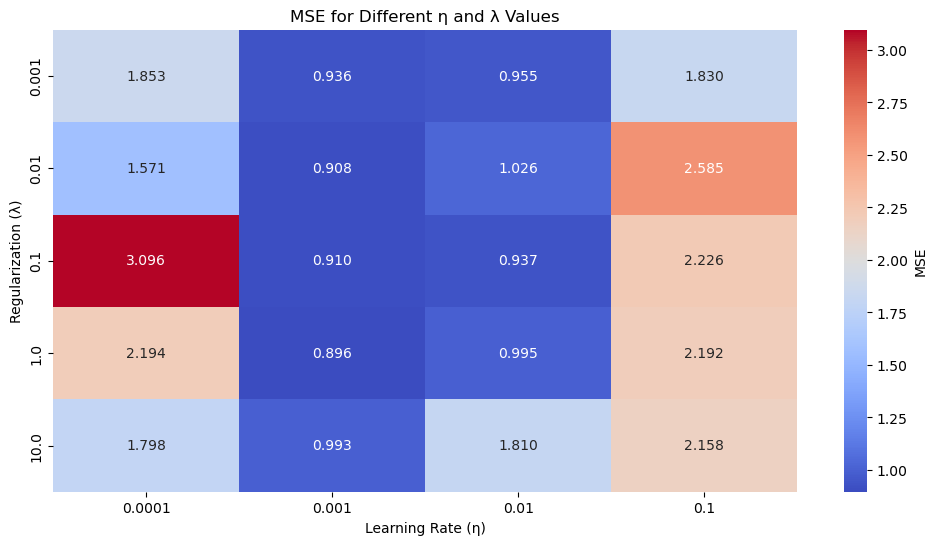
\includegraphics[width=0.9\linewidth]{MSE_Lambda_Learning_rate_TaskB_3.png}
    \caption{MSE for Different \(\eta\) and \(\lambda\)}
    \label{MSE_Lambda_Learning_rate_TaskB_3}
\end{figure}


The heatmap in Figure \ref{MSE_Lambda_Learning_rate_TaskB_3} shows the MSE for different combinations of learning rates (\(\eta\)) and regularization term (\(\lambda\)), illustrating the conditions that yield the best and worst performances. The results indicate that the best MSE values are achieved when learning rate is either \(0.001\) or \(0.01\). Specifically, with learning rate of \(0.001\), the \(\lambda\) values ranging from \(0.001\) to \(10.0\) provide consistently low MSE, indicating strong model performance. Similarly, with a learning rate of \(0.01\), \(\lambda\) values between \(0.001\) and \(1.0\) also produce low MSE values, showing a favorable balance of learning rate and regularization. Conversely, the worst MSE is observed when \(\lambda = 0.1\) and the learning rate is \(0.0001\), which is somewhat surprising given the generally stabilizing influence of a low learning rate. These findings highlight that while careful tuning of both \(\eta\) and \(\lambda\) is crucial, certain combinations like those with moderate regularization and appropriate learning rates, lead to more favorable results while others can unexpectedly degrade performance.


\begin{figure}[h!]
    \centering
    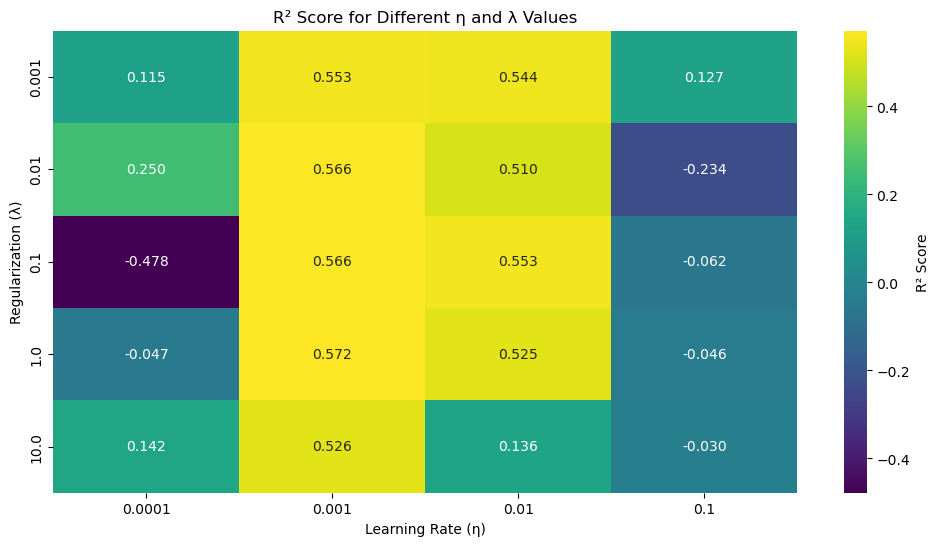
\includegraphics[width=0.9\linewidth]{R2_Score_Lambda_LearningRate_TaskB_4.png}
    \caption{\(R^2\) score across different \(\lambda\) and \(\eta\) values}
    \label{R2_Score_Lambda_LearningRate_TaskB_4}
\end{figure}

The heatmap in Figure \ref{R2_Score_Lambda_LearningRate_TaskB_4} shows \( R^2 \) scores for various combinations of learning rates (\(\eta\)) and regularization terms (\(\lambda\)), revealing both effective and poor parameter settings. The best \( R^2 \) values are achieved when \( \eta =0.001\), regardless of \(\lambda\), indicating stable and consistent model performance across different \(\lambda\) values. Similarly, when \( \eta = 0.01\), the \( R^2 \) scores are also good for \(\lambda\) values ranging from \(0.001\) to \(1.0\). In contrast, the worst performance occurs when \( \eta = 0.0001\) and \(\lambda = 0.1\), as well as when \(\eta = 0.1\) and \(\lambda = 0.01\). These settings result in negative \( R^2 \) scores, indicating that the model is either underfitting or struggling to converge properly. This highlights the importance of careful hyperparameter tuning. Choosing the wrong learning rates or regularization values can make the model perform poorly. Proper tuning helps find the right balance between learning effectively, being stable, and making good predictions on new data.


\subsection{Activation Function}


\begin{figure}[h!]
    \centering
    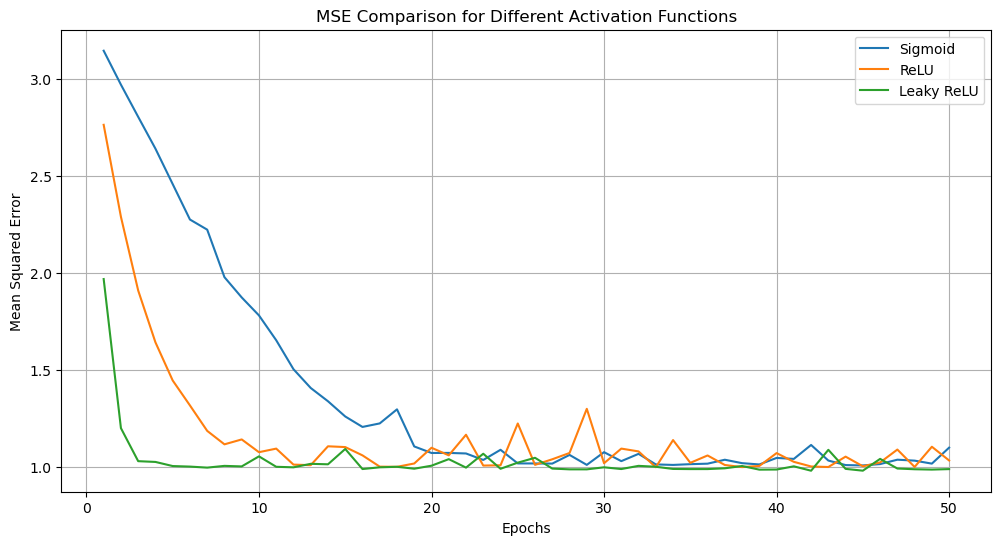
\includegraphics[width=0.9\linewidth]{TaskC_1.png}
    \caption{MSE Comparison for Different Activation Functions}
    \label{TaskC_1}
\end{figure}

The plot in Figure \ref{TaskC_1} shows the MSE over 50 epochs for Sigmoid, ReLU, and Leaky ReLU activation functions. Each activation function starts at a different MSE level. Sigmoid starts the highest, while Leaky ReLU starts the lowest. As training goes on, Sigmoids MSE decreases steadily but slowly, which could be due to the vanishing gradient problem. ReLU drops the MSE quickly at first but has several spikes along the way, showing instability, possibly because some neurons stopped updating. There are times when Sigmoids MSE even becomes lower than ReLUs. However, by the end, Sigmoid ends up with the highest MSE, while Leaky ReLU ends with the lowest. This means that Leaky ReLU not only starts better but also keeps reducing the error smoothly, making it the most effective choice overall.


\subsection{Classification}


\begin{figure}[h!]
    \centering
    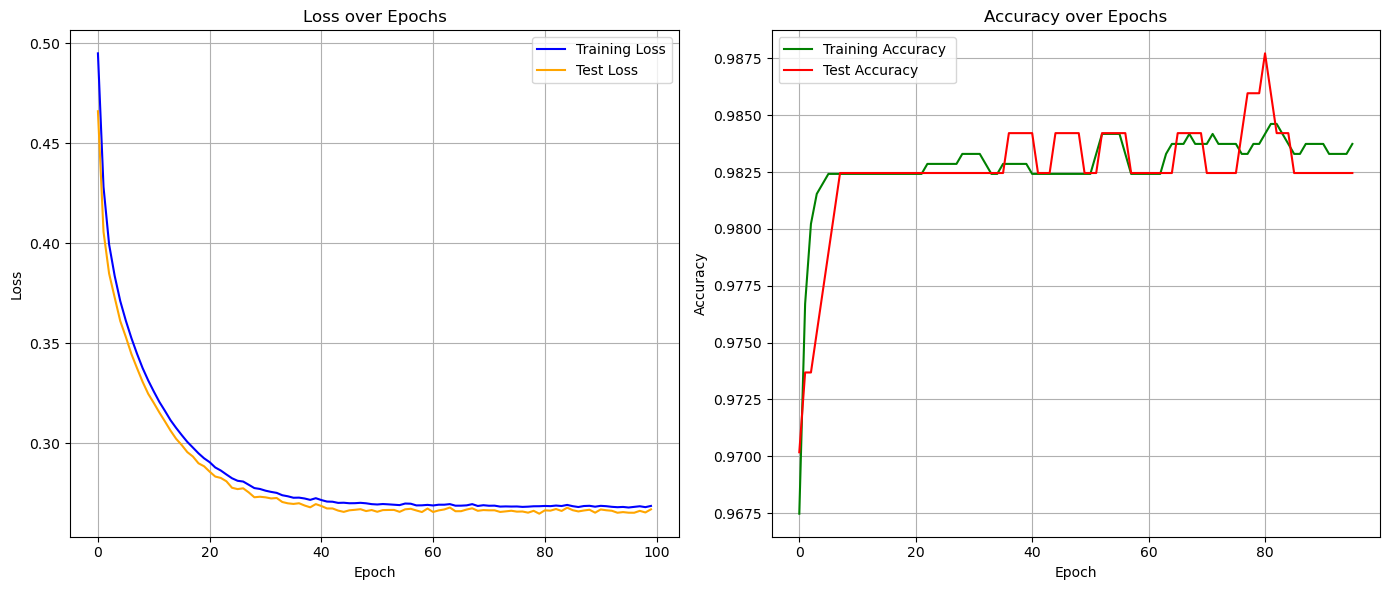
\includegraphics[width=1.2\linewidth]{Training_Val_loss_accuracy_TaskD.png}
    \caption{Loss and Accuracy over Epochs for Training and Test Data}
    \label{Training_Val_loss_accuracy_TaskD}
\end{figure}


Figure \ref{Training_Val_loss_accuracy_TaskD} presents two plots: The first shows the loss over epochs, and the second displays accuracy over epochs for both training and test datasets. In the loss plot, the training (blue line) and test (orange line) are almost identical throughout the epochs, indicating good consistency and generalization between the training and test data. However, in the accuracy plot, while the training accuracy (green line) remains relatively stable around 98\%, the test accuracy (red line) exhibits some peaks and fluctuations. These peaks indicate sensitivity to the test data, suggesting that while the model is learning effectively, it may occasionally overreact to the variations in the test set. This is why the accuracy plot is less stable compared to the smooth decline seen in the loss plot. These fluctuations could be mitigated by using additional regularization or further hyperparameter tuning to enhance stability, especially in test scenarios.



\begin{figure}[h!]
    \centering
    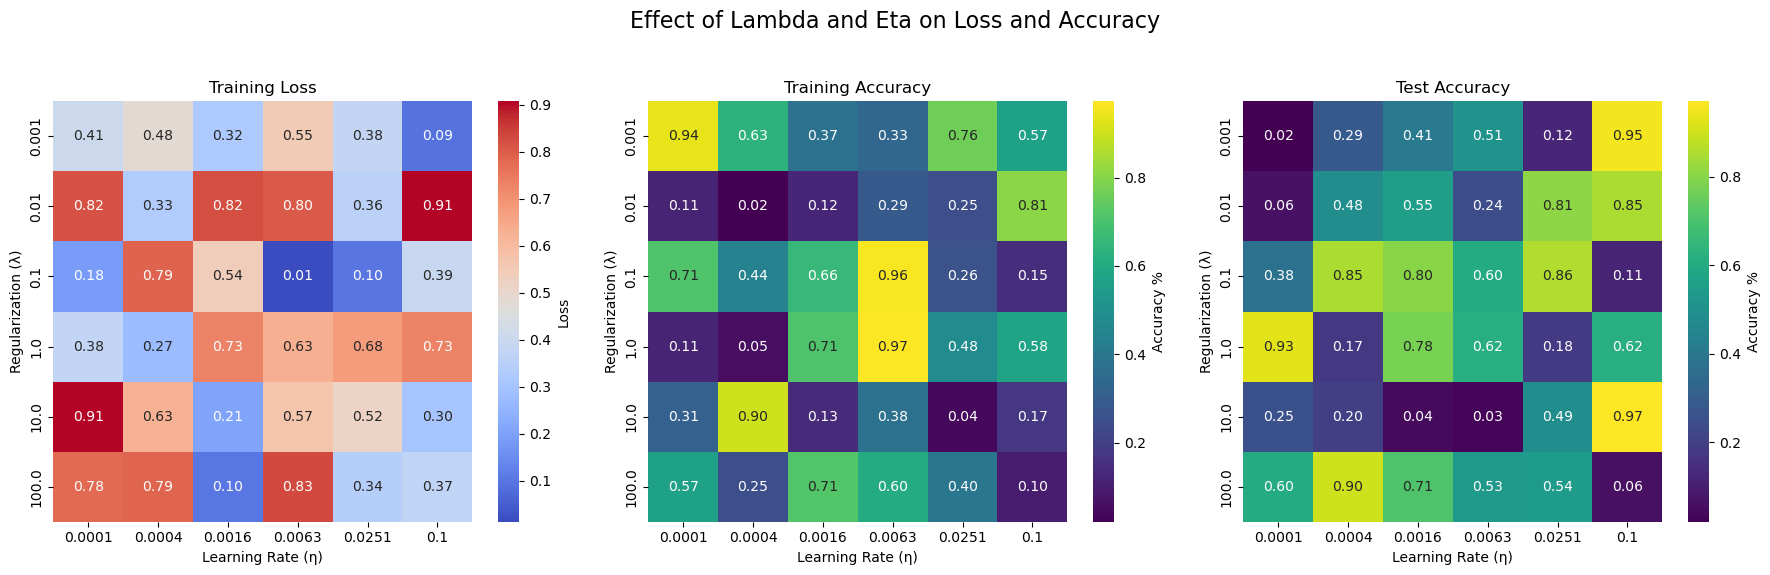
\includegraphics[width=1.2\linewidth]{Lambda_ETA_on_loss_Accuracy_TaskD_2.png}
    \caption{Effect of Lamda and Learning rate on Loss and Accuracy. (This figure has also been included individually in our GitHub repository to provide a clearer view of the values on the heatmap)}
    \label{Lambda_ETA_on_loss_Accuracy_TaskD_2}
\end{figure}




Figure \ref{Lambda_ETA_on_loss_Accuracy_TaskD_2} illustrates three plots: Training loss, Training accuracy, and Test accuracy for different combinations of learning rates (\(\eta\)) and regularization values (\(\lambda\)). These plots show how these hyperparameters impact the models performance, helping us understand which combinations yield the best results for both training and testing data. From the training loss heatmap, we see that \(\eta = 0.0063\) and \(\lambda = 0.1\) provide a low training loss, which corresponds to a high training accuracy of 0.96 and a decent test accuracy of 0.60. Another good combination is when \(\eta = 0.0063\) and \(\lambda = 1.0\), where training accuracy reaches 0.97, showing effective learning. However, our goal is to achieve the best possible test accuracy, and this occurs with \(\eta = 0.1\) and \(\lambda = 10\), giving a value of 0.97 for test accuracy. Although the training loss for this combination is 0.30, which is acceptable, the training accuracy is only 0.17, which is quite poor, indicating underfitting during training. Additionally, when \(\eta = 0.0016\) or \(\eta = 0.0063\) with \(\lambda = 0.1\) or \(1.0\), these combinations also give decent results, with very high training accuracy and acceptable training loss, though the test accuracy remains moderate. These results highlight the importance of balancing hyperparameters to ensure good training performance while also achieving strong generalization on test data.


\subsection{Logistic Regression}


\begin{figure}[h!]
    \centering
    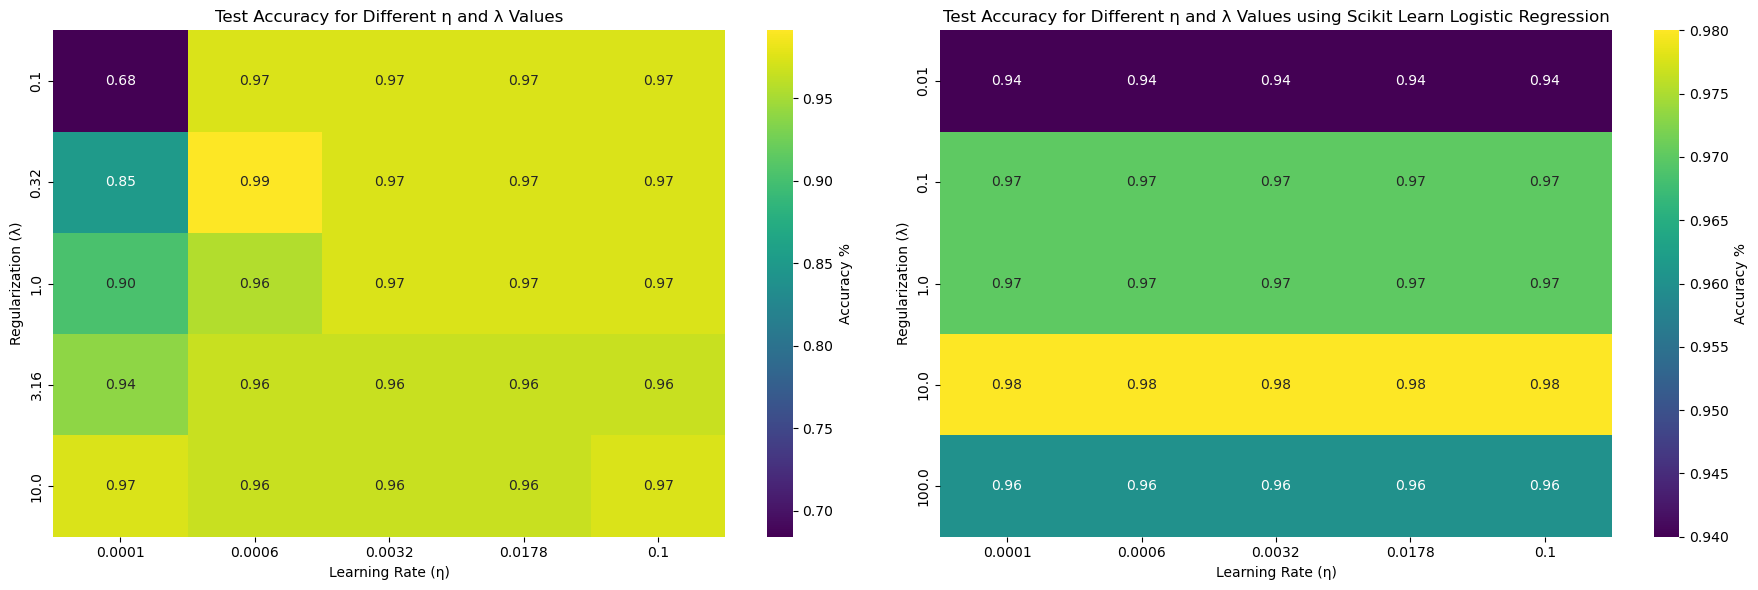
\includegraphics[width=1.2\linewidth]{Accuracy_taskE.png}
    \caption{Test Accuracy for Different learning rates and lamda values for own Logistic Regression and Scikit-Learn Logistic Regression.}
    \label{Accuracy_taskE}
\end{figure}


Figures \ref{Lambda_ETA_on_loss_Accuracy_TaskD_2} and \ref{Accuracy_taskE} illustrate the effect of different learning rates (\(\eta\)) and L2 regularization values (\(\lambda\)) on test accuracy for three models: the FFNN (Figure \ref{Lambda_ETA_on_loss_Accuracy_TaskD_2}), and the Custom and Scikit-Learn Logistic Regression models (Figure \ref{Accuracy_taskE}). For the FFNN, the best test accuracy (0.97) is achieved with \(\eta = 0.1\) and \(\lambda = 10\), though training accuracy is low, indicating underfitting. Other combinations, such as \(\eta = 0.0063\) with \(\lambda = 0.1\) or \(1.0\), yield high training accuracy and moderate test accuracy, underscoring the need for balanced hyperparameter tuning for optimal results.

For the Custom Logistic Regression model, results are best when the learning rate is high, generally performing well for all regularization values (\(\lambda\)) when the learning rate (\(\eta\)) ranges from 0.0006 to 0.1. This indicates that performance is more dependent on the learning rate than on \(\lambda\). In contrast, for Scikit-Learn's logistic regression, performance is more dependent on the regularization value, achieving the best results when \(\lambda = 10\) across all learning rates. Overall, the Custom Logistic Regression demonstrates a strong reliance on learning rate adjustments, while Scikit-Learn's logistic regression exhibits stability, particularly with moderate to high regularization values.




\section{Discussion}

In this study, we explored various algorithms, each demonstrating specific strengths and weaknesses that made them suitable for different parts of the project.

\subsection{Pros and Cons of the algorithms}


 Linear models, such as OLS and Ridge Regression, offered simplicity, capturing general trends effectively in linear data. Ridge, with its regularization, proved particularly useful in controlling noisy data, although too much regularization risked underfitting in some scenarios. FFNN proved effective at capturing non-linear relationships, especially when using activation functions like Leaky ReLU, which mitigated issues like vanishing gradients and dying neurons.

SGD and its variations, such as mini-batch and momentum, brought a significant advantage in terms of optimization speed. However, they introduced instability during learning, especially in scenarios with noisy gradient updates. For example, Figure \ref{MSE_OLS_plot_momentum_no_momentum} illustrates how, although momentum led to faster convergence, its benefits over plain SGD were not as substantial. FFNN is generally effective for non-linear relationships, also showed certain limitations. Figure \ref{TaskC_1} reveals that activation functions like ReLU experienced spikes in MSE, likely due to the "dying ReLU" problem, where neurons stop updating entirely. Even the better performing Leaky ReLU showed sensitivity to learning rates and required careful hyperparameter tuning, as seen in Figures \ref{Lambda_ETA_on_loss_Accuracy_TaskD_2} and \ref{Accuracy_taskE}, where imbalanced choices of learning rates and \(\lambda\) values led to poor model performance and underfitting in several cases. These results underscore the delicate trade-off between parameter tuning and model stability, particularly for more complex and adaptive neural architectures.

\subsection{Regression}

The best-performing algorithm for regression in this study was Ridge Regression. As shown in Figure \ref{Results_Obtained_linear_and_NN_code_taskB_1}, Ridge achieved the lowest MSE and highest \( R^2 \) scores, unexpectedly outperforming the MLPRegressor, which is typically more suited to non-linear relationships. This advantage is likely due to Ridge’s regularization term (\(\lambda\)), which helps stabilize the model by penalizing large coefficients, enhancing its ability to generalize.

The tuning of hyperparameters, specifically learning rate (\(\eta\)) and regularization (\(\lambda\)), proved crucial in optimizing Ridge's performance. From Figures \ref{MSE_Lambda_Learning_rate_TaskB_3} and \ref{R2_Score_Lambda_LearningRate_TaskB_4}, the lowest MSE (0.896) and the highest \( R^2 \) score (0.572) were achieved with \(\lambda = 1.0\) and \(\eta = 0.001\). These values surpass those seen in other models, confirming that, in this specific context, Ridge offered the best balance between minimizing error and explaining data variance, even though MLPRegressor might typically be expected to perform better in capturing non-linear patterns.


\subsection{Classification}

Based on the results, the best algorithm for classification was the Scikit-Learn Logistic Regression model. As shown in Figure \ref{Accuracy_taskE}, this model achieved consistently high test accuracy across a range of learning rates and regularization values (\(\lambda\)), demonstrating both stability and adaptability. Specifically, the Scikit-Learn Logistic Regression model performed best with \(\lambda = 10\), achieving the highest accuracy, which indicates that its performance was more dependent on regularization than on the learning rate.

In comparison, the custom Logistic Regression model was more sensitive to learning rate adjustments and performed well with higher learning rates across multiple values of \(\lambda\). However, it did not consistently achieve the same high accuracy as the Scikit-Learn implementation. Additionally, the Feed-Forward Neural Network (FFNN) achieved a high test accuracy of 0.97 with \(\eta = 0.1\) and \(\lambda = 10\), but this setting led to low training accuracy, indicating possible underfitting. Overall, Scikit-Learn's Logistic Regression model demonstrated the most reliable performance for classification, with robust generalization across the test data.




\section{Conclusion}

This study demonstrated that Ridge Regression performed best for regression tasks, benefiting from its regularization term to achieve the lowest MSE and highest \( R^2 \) scores, even surpassing the MLPRegressor. Key parameters, \(\lambda = 1.0\) and \(\eta = 0.001\), were essential in minimizing error and enhancing data variance explanation, underscoring the importance of tuning for optimal results. In classification, Scikit-Learn's Logistic Regression showed consistently high accuracy, especially at \(\lambda = 10\), proving to be both stable and adaptable compared to the more sensitive custom Logistic Regression model and the Feed-Forward Neural Network (FFNN).

Each algorithm had specific strengths and limitations. Linear models like OLS offered simplicity and good generalization for basic trends but struggled with more complex, non-linear patterns. Techniques like mini-batch and momentum in SGD helped speed up optimization, though they ultimately produced nearly the same results. Future work could focus on deeper neural networks, robust optimization methods, and automated hyperparameter tuning using gridsearchCV, to enhance stability and performance, especially for tasks with complex, non-linear data relationships.


\section{Acknowledgment}


During this project, we gathered essential information for both the code and theoretical concepts from Professor Morten Hjorth-Jensen’s GitHub page and the extra materials and videos he provided.


The ChatGPT tool has been valuable a lot during this project. It has been used to:
\begin{itemize}
    \item Provided guidance on adapting and modifying code when encountering issues, especially with generating plots, and for the feed-forward neural network.

    \item Review and refined the grammar, enhancing the overall clarity and language of the project.

\end{itemize}





\printbibliography





\section{Appendix}


\url{https://github.uio.no/arangans/Project2_0.git}





\end{document}
